% ============================================================
%  FEA_notation_intuition.tex   --  STANDALONE.
%  Does not \input anything.  Build:  pdflatex FEA_notation_intuition.tex
% ============================================================
\documentclass[11pt]{article}

\usepackage[letterpaper,margin=1in,headheight=14pt]{geometry}
\usepackage[T1]{fontenc}
\usepackage{amsmath,amssymb}
\usepackage{booktabs}
\usepackage{array}
\usepackage{enumitem}
\usepackage{tikz}
\usetikzlibrary{arrows.meta}
\usepackage{fancyhdr}
\usepackage{xcolor}
\usepackage[most]{tcolorbox}
\usepackage[colorlinks=true,linkcolor={blue!45!black},pdfborder={0 0 0}]{hyperref}

\definecolor{IntFrame}{HTML}{1F6F8B}
\definecolor{PitFrame}{HTML}{B23A3A}
\definecolor{MEFrame} {HTML}{2E7D4F}

\pagestyle{fancy}\fancyhf{}
\fancyhead[L]{\small\sffamily FEA notation and intuition}
\fancyhead[R]{\small\sffamily\thepage}
\renewcommand{\headrulewidth}{0.4pt}

\newcommand{\dx}{\,\mathrm{d}x}
\newcommand{\ip}[2]{\bigl\langle #1,\,#2\bigr\rangle}
\newcommand{\norm}[1]{\lVert #1\rVert}
\newcommand{\Vh}{V_{h}}
\newcommand{\Kmat}{\bm{K}}
\usepackage{bm}
\setlength{\parindent}{0pt}

\newlist{pts}{itemize}{1}
\setlist[pts]{label=\textbullet, leftmargin=1.25em, topsep=3pt,
              itemsep=3.5pt, parsep=0pt}

\tcbset{basebox/.style={enhanced,breakable,sharp corners=downhill,boxrule=0.8pt,
  left=8pt,right=8pt,top=6pt,bottom=6pt,
  fonttitle=\bfseries\sffamily\small,
  attach boxed title to top left={xshift=8pt,yshift=-\tcboxedtitleheight/2},
  boxed title style={sharp corners,boxrule=0pt,size=small},toptitle=2pt}}
\newtcolorbox{intuition}[1][]{basebox,colback=IntFrame!6,colframe=IntFrame,
  coltitle=white,colbacktitle=IntFrame,title={Intuition#1}}
\newtcolorbox{pitfall}[1][]{basebox,colback=PitFrame!5,colframe=PitFrame,
  coltitle=white,colbacktitle=PitFrame,title={Watch out#1}}
\newtcolorbox{worked}[1][]{basebox,colback=MEFrame!5,colframe=MEFrame,
  coltitle=white,colbacktitle=MEFrame,title={Check it by hand#1}}

\title{\bfseries FEA notation, assembled in order\\[0.35em]
  \large residual, test, trial, shape function, Galerkin,\\
  the dot product, and Galerkin orthogonality}
\author{Hasan}
\date{\today}

\begin{document}
\maketitle
\thispagestyle{fancy}

\noindent
Two running examples, so nothing stays abstract:

\begin{center}\small
\renewcommand{\arraystretch}{1.4}
\begin{tabular}{@{}l>{\raggedright\arraybackslash}p{0.72\linewidth}@{}}
\toprule
\textbf{Example A} & $-u''+q(x)u=f$ on $(-\pi,\pi)$, periodic, with
  $q=3-\sin x-\sin 2x-\cos x$, \ $f=2e^{\sin x}e^{\cos x}$, \
  exact $u=e^{\sin x}e^{\cos x}$. Used for the numbers.\\
\textbf{Example B} & $-u''=2$ on $(0,1)$, $u(0)=u(1)=0$, exact $u=x(1-x)$.
  Two hat functions, one unknown. Worked by hand in \S\ref{sec:worked}.\\
\textbf{Example C} & The same BVP, but the space is
  $V_h=\operatorname{span}\{\sin\pi x\}$ --- still one unknown, but $u$ is
  \emph{not} in the space, so the error is visible. The whole chain is walked
  on it in \S\ref{sec:chainex}.\\
\bottomrule
\end{tabular}
\end{center}

% ==================================================================
\section{The residual $R$ --- the thing you are trying to kill}

Move everything to one side and feed it \emph{any} candidate function $w$:
\[
  \boxed{\;R(w)(x)=-w''(x)+q(x)\,w(x)-f(x)\;}
\]

\begin{pts}
\item $R$ measures how badly $w$ fails the equation, \textbf{point by point}.
\item $R(u)\equiv0$. That is exactly what ``$u$ is the exact solution'' means.
\item For anything you can actually compute, $R\neq0$ somewhere.
\end{pts}

\subsection*{Why $w$, not $u$}

\begin{pts}
\item $u$ is reserved: it means \emph{the} exact solution, one specific function.
\item $R$ must accept \emph{any} candidate. $R(u)$ only ever describes the
      answer you do not have --- and equals zero, so it says nothing.
\item $w$ is a placeholder: ``whatever function you hand me''.
\end{pts}

\subsection*{Reading the brackets}

$R$ is an \textbf{operator}: a function goes in, a function comes out.

\begin{center}\small
\renewcommand{\arraystretch}{1.35}
\begin{tabular}{@{}lll@{}}
\toprule
\textbf{written} & \textbf{what it is} & \textbf{compare} \\
\midrule
$R$       & the operator. ``the residual''                  & $D$, differentiation \\
$R(w)$    & a \textbf{function} of $x$                      & $D(w)=w'$ \\
$R(w)(x)$ & a \textbf{number}: its value at the point $x$   & $D(w)(x)=w'(x)$ \\
\bottomrule
\end{tabular}
\end{center}

\begin{pts}
\item $R(x)(w)$ is \textbf{wrong}. The order is not free: you must supply the
      function first --- there is nothing to differentiate until you do --- and
      only then the point.
\item $R(x)$ alone is loose shorthand. It hides \emph{which} candidate produced
      it. Fine in prose when the candidate is obvious, ambiguous in a definition.
\end{pts}

\medskip
\textbf{Same operator, three different candidates} (Example A):

\begin{center}\small
\renewcommand{\arraystretch}{1.2}
\begin{tabular}{@{}rccc@{}}
\toprule
$x$ & $R(u)(x)$ & $R(w_1)(x)$ & $R(w_2)(x)$\\
    & \emph{exact} & $w_1=1$  & $w_2=\cos x$\\
\midrule
$-2.0$ & $0$              & $3.037$  & $-2.433$\\
$-1.0$ & $4\cdot10^{-16}$ & $2.731$  & $1.335$\\
$ 0.0$ & $0$              & $-3.437$ & $-2.437$\\
$ 1.0$ & $0$              & $-7.255$ & $-7.041$\\
$ 2.0$ & $0$              & $-0.011$ & $-5.049$\\
\bottomrule
\end{tabular}
\end{center}

\begin{pts}
\item $R(u)$ is the zero \emph{function}; $R(w_1)$ is a different function,
      not zero; $R(w_1)(0)=-3.437$ is a single \emph{number}.
\item $R(w_1)(2)=-0.011$: a wrong candidate can be accidentally right at a
      point. $R$ small \emph{somewhere} means nothing.
\end{pts}

% ==================================================================
\section{Why you cannot kill $R$ everywhere}

\begin{pts}
\item ``$R(w)(x)=0$ at every $x$'' is \textbf{infinitely many} conditions, one
      per point.
\item You have \textbf{finitely many} unknowns.
\item So do not kill $R$ everywhere. Kill a \emph{finite number of weighted
      averages} of it.
\end{pts}

% ==================================================================
\section{Test function --- the probe}

Pick a weight function $v$ and demand
\[
  \int R(W)\,v\dx = 0 .
\]

\begin{pts}
\item Meaning: \emph{$R$ has no component along $v$}. Not that $R$ is zero ---
      only that $v$ cannot detect it.
\item $v$ is the \textbf{test function}: a probe, a measuring device.
\item \textbf{One test function $=$ one equation.} Choose $M+1$ of them and you
      get $M+1$ equations for $M+1$ unknowns. That is the entire design.
\end{pts}

% ==================================================================
\section{Trial function --- the candidate}

The thing you solve \emph{for}, restricted to a chosen form:
\[
  U(x)=\xi_0\varphi_0(x)+\xi_1\varphi_1(x)+\dots+\xi_M\varphi_M(x).
\]

\begin{center}\small
\begin{tabular}{@{}ll@{}}
\toprule
\textbf{trial} & what you build the answer out of\\
\textbf{test}  & what you probe the leftover with\\
\bottomrule
\end{tabular}
\end{center}

\begin{pitfall}[: they are not opposites]
Trial and test are two \emph{jobs}, not two ends of something. They are not
perpendicular to each other --- and in the method below they are drawn from the
same set of functions.
\end{pitfall}

% ==================================================================
\section{``Galerkin'' --- one specific choice}

You must decide which functions to use as tests:

\begin{center}\small
\renewcommand{\arraystretch}{1.25}
\begin{tabular}{@{}ll@{}}
\toprule
\textbf{Galerkin}        & test space $=$ trial space \\
\textbf{Petrov--Galerkin}& test space $\neq$ trial space \\
\bottomrule
\end{tabular}
\end{center}

\begin{pts}
\item \textbf{That is the entire content of the word ``Galerkin''.} Nothing more.
\item Both examples here are Galerkin: tests and trials both come from
      $\operatorname{span}\{\varphi_0,\dots,\varphi_M\}$.
\end{pts}

% ==================================================================
\section{$N$ versus $\varphi$ versus ``shape function''}

Same objects, two levels of bookkeeping.

\begin{pts}
\item \textbf{$N$ --- local, per element.} On one element mapped to
      $0\le\xi\le1$, a 2-node linear element has $N_0(\xi)=1-\xi$,
      $N_1(\xi)=\xi$. Two functions on one element.
\item \textbf{$\varphi_i$ --- global, per node.} Hold every node at zero, lift
      node $i$ to $1$, join with straight lines.
\item \textbf{Relation:} $\varphi_i$ is just the local $N$'s that touch node
      $i$, stitched together.
\item \textbf{``Shape function''} is the engineering word --- usually $N$
      (local), sometimes $\varphi$ (global). Same functions.
\end{pts}

\begin{center}
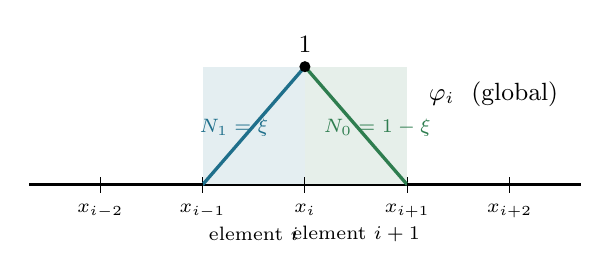
\begin{tikzpicture}[>=Latex,scale=1.0]
  \fill[IntFrame!12] (1.8,0) rectangle (3.1,1.5);
  \fill[MEFrame!12]  (3.1,0) rectangle (4.4,1.5);
  \draw[thick] (-0.4,0) -- (6.6,0);
  \foreach \i/\lab in {0.5/{x_{i-2}},1.8/{x_{i-1}},3.1/{x_i},4.4/{x_{i+1}},5.7/{x_{i+2}}}{
     \draw (\i,-0.1) -- (\i,0.1);
     \node[below,font=\scriptsize] at (\i,-0.12) {$\lab$};}
  \draw[very thick,IntFrame] (1.8,0) -- (3.1,1.5);
  \draw[very thick,MEFrame]  (3.1,1.5) -- (4.4,0);
  \draw[very thick] (-0.4,0) -- (1.8,0);
  \draw[very thick] (4.4,0) -- (6.6,0);
  \fill (3.1,1.5) circle (2pt);
  \node[above,font=\small] at (3.1,1.55) {$1$};
  \node[right,font=\small] at (4.55,1.15) {$\varphi_i$ \ (global)};
  \node[font=\scriptsize,IntFrame] at (2.2,0.72) {$N_1=\xi$};
  \node[font=\scriptsize,MEFrame]  at (4.02,0.72) {$N_0=1-\xi$};
  \node[font=\scriptsize] at (2.45,-0.62) {element $i$};
  \node[font=\scriptsize] at (3.75,-0.62) {element $i+1$};
\end{tikzpicture}
\par\smallskip
{\small On the element \emph{left} of node $i$, node $i$ is the right node, so
it carries $N_1=\xi$. On the element \emph{right} of it, node $i$ is the left
node, so it carries $N_0=1-\xi$. Zero on every other element.}
\end{center}

Two properties are the reason this basis is used:

\begin{pts}
\item $\varphi_i(x_j)=1$ if $i=j$, else $0$. So in $U=\sum_j\xi_j\varphi_j$ each
      coefficient $\xi_j$ \textbf{is} the nodal value $U(x_j)$ --- the unknowns
      are the displacements themselves, no transformation.
\item $\varphi_i$ is nonzero on only \textbf{two} elements, so $\varphi_i$ and
      $\varphi_j$ overlap only for neighbours. That is where sparsity comes from.
\end{pts}

% ==================================================================
\section{The dot product --- and where it comes from}

\begin{pts}
\item \textbf{Vectors:} $\bm{a}\cdot\bm{b}=a_1b_1+a_2b_2+\cdots$ --- multiply
      matching components, add.
\item \textbf{Functions:} $\int v\,w\dx$ --- multiply at each $x$, add over $x$.
      Same operation, continuous index.
\end{pts}

The pairing you actually use is \textbf{not invented}. It falls out of the test
equation after one integration by parts:
\begin{align*}
  \int R(U)\,v\dx &= 0\\
  \int\bigl(-U''+qU-f\bigr)v\dx &= 0\\
  \underbrace{\int\bigl(U'v'+q\,U\,v\bigr)\dx}_{\textstyle\text{call this }\ip{U}{v}}
    \;-\;\underbrace{\bigl[U'v\bigr]}_{=\,0\ \text{at the ends}}
    \;-\;\int f\,v\dx &= 0
\end{align*}
\[
  \boxed{\;\ip{v}{w}:=\int\bigl(v'w'+q\,v\,w\bigr)\dx\;}
  \qquad\text{(Example B has $q=0$, so $\ip{v}{w}=\int v'w'\dx$)}
\]

\begin{pts}
\item \textbf{It is a genuine dot product.} The integrand is
      $\bigl[v',\sqrt{q}\,v\bigr]\cdot\bigl[w',\sqrt{q}\,w\bigr]$ --- an
      ordinary 2-component dot product at each $x$, summed over $x$.
\item Symmetric; linear in each slot; and
      $\ip{v}{v}=\int\bigl[(v')^2+qv^2\bigr]\dx>0$ unless $v\equiv0$. Exactly
      the properties of $\bm{a}\cdot\bm{b}$.
\end{pts}

\begin{intuition}[: what integrating by parts bought]
The original $R$ needs $U''$. After moving one derivative onto $v$, only $U'$
appears. That is what makes a piecewise-linear $U$ --- which has no second
derivative at all --- a legal candidate.
\end{intuition}

% ==================================================================
\section{Orthogonality --- the generic word}

\begin{pts}
\item $\ip{a}{b}=0$ means \textbf{$a$ has no component along $b$}. Perpendicular.
\item Exactly as with vectors. Nothing FEM-specific about the word itself.
\end{pts}

% ==================================================================
\section{\texorpdfstring{Testing with each $\varphi_i$ \emph{is} $\Kmat\bm{\xi}=\bm{b}$}{Testing with each phi\_i is K xi = b}}

Use $v=\varphi_i$, one at a time, $i=0,\dots,M$:
\begin{align*}
  \ip{U}{\varphi_i} &= \int f\,\varphi_i\dx
     && \text{one equation per test function}\\
  \Bigl\langle\textstyle\sum_j\xi_j\varphi_j,\ \varphi_i\Bigr\rangle
     &= \int f\,\varphi_i\dx
     && \text{substitute }U=\textstyle\sum_j\xi_j\varphi_j\\
  \sum_j \xi_j\,\ip{\varphi_j}{\varphi_i} &= \int f\,\varphi_i\dx
     && \text{linear in the first slot}
\end{align*}
which is row $i$ of a matrix system:
\[
  \boxed{\;K_{ij}=\ip{\varphi_j}{\varphi_i},\qquad
         b_i=\int f\,\varphi_i\dx,\qquad \Kmat\bm{\xi}=\bm{b}\;}
\]

\begin{pts}
\item $\Kmat$ is the \textbf{table of pairings of the basis functions with each
      other}. Checked on Example A: $\max_{ij}\bigl|K_{ij}-\ip{\varphi_j}{\varphi_i}\bigr|
      =2.2\times10^{-16}$.
\item Its diagonal is $\ip{\varphi_i}{\varphi_i}$ --- large and positive
      ($4.879,\ 4.722,\ 4.513,\dots$ on a $7\times7$ case).
\item So the $\varphi$'s are emphatically \textbf{not} orthogonal to one
      another. If they were, $\Kmat$ would be the zero matrix and there would be
      nothing to solve.
\end{pts}

% ==================================================================
\section{Galerkin orthogonality}

\begin{pts}
\item The exact $u$ satisfies the identity for \emph{every} admissible $v$,
      including each $\varphi_i$: \ $\ip{u}{\varphi_i}=\int f\varphi_i\dx$.
\item Row $i$ of your system says \ $\ip{U}{\varphi_i}=\int f\varphi_i\dx$.
\item Subtract. \textbf{The load cancels.} With the error $e:=u-U$:
\end{pts}
\[
  \boxed{\;\ip{e}{\varphi_i}=0,\qquad i=0,1,\dots,M\;}
\]

\begin{center}\small
\renewcommand{\arraystretch}{1.3}
\begin{tabular}{@{}ll@{}}
\toprule
\textbf{Galerkin} & it holds because the tests were taken from the trial
                    space --- which is how $U$ was built\\
\textbf{orthogonality} & the pairing is zero\\
\bottomrule
\end{tabular}
\end{center}

\subsection*{Why the two sides are equal --- they get there differently}

The subtraction looks empty: two identical numbers giving zero. The content is
in \emph{why} each side reaches that number.

\begin{center}\small
\renewcommand{\arraystretch}{1.4}
\begin{tabular}{@{}l>{\raggedright\arraybackslash}p{0.68\linewidth}@{}}
\toprule
$\ip{u}{\varphi_i}=\int f\varphi_i$
  & because $u$ solves the problem against \emph{every} test function, and
    $\varphi_i$ happens to be one of them. $u$ had no choice; nobody arranged
    this.\\
$\ip{U}{\varphi_i}=\int f\varphi_i$
  & because you \textbf{forced} it. This is the equation you imposed:
    $\ip{U}{\varphi_i}=\Kmat\bm{\xi}=\bm{b}=\int f\varphi_i$.\\
\bottomrule
\end{tabular}
\end{center}

\begin{pts}
\item One side is a \emph{property} of the true solution; the other is a
      \emph{constraint you built in}. They reach the same number from opposite
      directions.
\item You did not know $\ip{u}{\varphi_i}$ at the start. You could compute
      $\int f\varphi_i$ from $f$ alone --- so you learned one true number about
      $u$ without knowing $u$. Then you chose $\bm{\xi}$ to reproduce it.
\item \textbf{That is the accomplishment:} $M+1$ quantities of the unknown
      solution, matched \emph{exactly}, paid for with $f$ alone.
\item Why rewrite it as $\ip{e}{\varphi_i}=0$? Same fact, usable form ---
      compare $x=5$ with $x-5=0$. The second is what you substitute into other
      equations, and it is exactly what deletes a term later:
      \[
        \norm{e}_E^{2}=\ip{e}{u-U}=\ip{e}{u-v}
          +\underbrace{\ip{e}{v-U}}_{=\,0,\ v-U\in\Vh}=\ip{e}{u-v}.
      \]
\end{pts}

\begin{intuition}[: one scale]
You own one scale; it reports one number.
\begin{pts}
\item From the spec sheet ($f$) you know the true object must read $1.273$ ---
      without ever putting it on the scale.
\item You tune your model until \emph{it} reads $1.273$.
\item Now weigh the difference between them: $\mathbf{0.000}$.
\end{pts}
The difference is not absent --- the two objects genuinely differ. It is
\emph{unmeasurable by that scale}. Your instrument cannot tell them apart.
\end{intuition}

\begin{pitfall}[: what is orthogonal to what]
Galerkin orthogonality is \textbf{the error against the test functions},
$\ip{e}{\varphi_i}=0$. It is \emph{not} trial against test,
$\ip{\varphi_i}{\varphi_j}$ --- those are the entries of $\Kmat$, and they are
nonzero. Two different objects: $\Kmat$ is built from the nonzero one, the
theorem is about the zero one.
\end{pitfall}

\textbf{Measured on Example A}, $M=24$, so $25$ basis functions:

\begin{center}\small
\renewcommand{\arraystretch}{1.2}
\begin{tabular}{@{}ll@{}}
\toprule
$\max_i\bigl|\ip{e}{\varphi_i}\bigr|$ over all $25$ & $7.2\times10^{-14}$ \quad (machine zero)\\
$\ip{e}{\sin 2x}$ & $0.156$\\
$\ip{e}{\cos 3x}$ & $-0.125$\\
$\ip{e}{e}$       & $0.171$\\
\bottomrule
\end{tabular}
\end{center}

\begin{pts}
\item \textbf{What it does not say.} $\ip{e}{\varphi_i}=0$ is $M+1$ numbers;
      $e$ is a whole function. $M+1$ numbers cannot determine it --- which is
      why $e$ stays nonzero everywhere while every pairing is exactly zero.
      You learn $e$'s \emph{direction}, never its \emph{size}.
\end{pts}

\begin{intuition}[: the error is not small --- it is invisible]
Think of the $M+1$ basis functions as $M+1$ \textbf{sensors}. The only
measurement the solver ever performs on a function is $\ip{\cdot}{\varphi_i}$ ---
that is what assembling a row does. All $25$ sensors read zero on $e$; an
outside probe reads $0.156$. The error sticks straight out of the space the mesh
can represent.

It has to: if any sensor had read nonzero, one row of $\Kmat\bm{\xi}=\bm{b}$
would be violated, and $\bm{\xi}$ would not be the solution.
\end{intuition}

\begin{center}
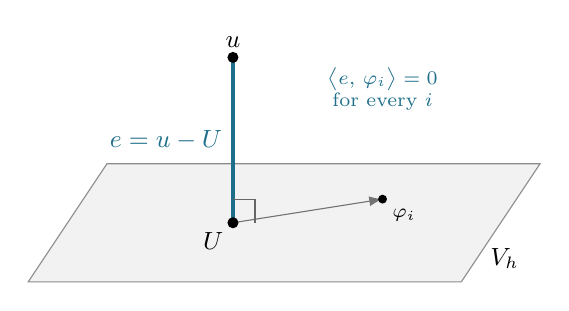
\begin{tikzpicture}[>=Latex,scale=1.0]
  \draw[fill=black!5,draw=black!45] (-2.6,-0.75) -- (2.9,-0.75)
        -- (3.9,0.75) -- (-1.6,0.75) -- cycle;
  \node[font=\small] at (3.45,-0.45) {$\Vh$};
  \coordinate (U) at (0,0);
  \coordinate (u) at (0,2.1);
  \coordinate (p) at (1.9,0.3);
  \draw[very thick,IntFrame] (u) -- (U)
        node[midway,left,font=\small,IntFrame] {$e=u-U$};
  \draw[black!55,->] (U) -- (p);
  \fill (U) circle (2pt); \node[below left,font=\small] at (U) {$U$};
  \fill (u) circle (2pt); \node[above,font=\small]      at (u) {$u$};
  \fill (p) circle (1.6pt); \node[below right,font=\scriptsize] at (p) {$\varphi_i$};
  \draw[black!60] (0,0.3) -- (0.28,0.3) -- (0.28,0);
  \node[font=\scriptsize,align=center,IntFrame] at (1.9,1.7)
       {$\ip{e}{\varphi_i}=0$\\ for every $i$};
\end{tikzpicture}
\par\smallskip
{\small $\Vh$ is everything the mesh can represent; the $\varphi_i$ are its
axes. $e$ has zero component along every axis.}
\end{center}

% ==================================================================
\section{Everything above, by hand}\label{sec:worked}

\begin{worked}[: Example B, one unknown]
$-u''=2$ on $(0,1)$, $u(0)=u(1)=0$. Exact solution $u=x(1-x)$. Here $q=0$, so
$\ip{v}{w}=\int_0^1 v'w'\dx$.

\textbf{Mesh:} two elements, $h=\tfrac12$, one free node at $x_1=\tfrac12$. So
$\Vh=\operatorname{span}\{\varphi_1\}$ --- exactly \emph{one} unknown $\xi_1$
and \emph{one} test function.
\[
  \varphi_1(x)=\begin{cases}2x, & 0\le x\le\tfrac12\\[2pt] 2(1-x), & \tfrac12\le x\le1\end{cases}
  \qquad
  \varphi_1'(x)=\begin{cases}+2, & 0<x<\tfrac12\\[2pt] -2, & \tfrac12<x<1\end{cases}
\]

\textbf{The matrix (one entry).}
\[
  K_{11}=\ip{\varphi_1}{\varphi_1}=\int_0^1(\varphi_1')^2\dx
        =2^2\cdot\tfrac12+(-2)^2\cdot\tfrac12=\boxed{4}
\]

\textbf{The load (one entry).} $\int_0^1 2\varphi_1\dx = 2\times(\text{area of the hat})
=2\times\tfrac12\cdot1\cdot1=\boxed{1}$

\textbf{Solve.} $4\xi_1=1\Rightarrow \xi_1=\tfrac14$. And indeed
$u(\tfrac12)=\tfrac12\cdot\tfrac12=\tfrac14$ --- exact at the node.

\medskip
\textbf{Now check Galerkin orthogonality by hand.} With $u'=1-2x$ and
$U'=\pm\tfrac12$:
\[
  \ip{u}{\varphi_1}=\int_0^{1/2}\!\!(1-2x)(2)\dx+\int_{1/2}^{1}\!\!(1-2x)(-2)\dx
   =\tfrac12+\tfrac12=1
\]
\[
  \ip{U}{\varphi_1}=\int_0^{1/2}\!\!(\tfrac12)(2)\dx+\int_{1/2}^{1}\!\!(-\tfrac12)(-2)\dx
   =\tfrac12+\tfrac12=1
\]
\[
  \Longrightarrow\quad \ip{e}{\varphi_1}=1-1=\boxed{0}
\]

\medskip
\textbf{But the error is not zero.} $e=u-U$:
\begin{center}\small
\begin{tabular}{@{}cccc@{}}
\toprule
$x$ & $u(x)$ & $U(x)$ & $e(x)$\\
\midrule
$0.25$ & $0.1875$ & $0.1250$ & $0.0625$\\
$0.50$ & $0.2500$ & $0.2500$ & $0$\\
$0.75$ & $0.1875$ & $0.1250$ & $0.0625$\\
\bottomrule
\end{tabular}
\end{center}
\[
  \ip{e}{e}=\int_0^1(e')^2\dx=\tfrac{1}{12}\approx0.0833\;\neq\;0,
  \qquad
  \ip{e}{\sin\pi x}=0.273\;\neq\;0 .
\]

\textbf{Read it:} $\ip{e}{\varphi_1}=0$ exactly, while $\ip{e}{e}=\tfrac1{12}$
and $\ip{e}{\sin\pi x}=0.273$. The error is a real, sizeable function --- it is
only the \emph{one} probe the mesh owns that cannot see it.
\end{worked}

% ==================================================================
\section{The whole chain, walked on one unknown}\label{sec:chainex}

\begin{worked}[: Example C --- one unknown, and a visible error]
Same BVP as Example B: $-u''=2$ on $(0,1)$, $u(0)=u(1)=0$, exact $u=x(1-x)$.
But now take the space
\[
  \varphi(x)=\sin\pi x,\qquad \Vh=\operatorname{span}\{\varphi\},
  \qquad U=\xi\,\varphi .
\]
One unknown $\xi$. Note $u=x(1-x)$ is \emph{not} a multiple of $\sin\pi x$, so
there will be a genuine error --- which is the point. Here $q=0$, so
$\ip{v}{w}=\int_0^1 v'w'\dx$.

\medskip
\textbf{$\rightarrow$ $R$ is the leftover.}
\ $R(U)=-U''-2=\xi\pi^{2}\sin\pi x-2$, an honest function of $x$:
\begin{center}\small
\begin{tabular}{@{}cccc@{}}
\toprule
$\xi$ & $R(0.25)$ & $R(0.50)$ & $R(0.75)$ \\
\midrule
$0.0000$ & $-2.0000$ & $-2.0000$ & $-2.0000$ \\
$0.2580$ & $-0.1995$ & $\phantom{-}0.5464$ & $-0.1995$ \\
$1.0000$ & $\phantom{-}4.9789$ & $\phantom{-}7.8696$ & $\phantom{-}4.9789$ \\
\bottomrule
\end{tabular}
\end{center}

\textbf{$\rightarrow$ Cannot kill it everywhere.}
$\xi\pi^{2}\sin\pi x-2=0$ needs $\xi=2/(\pi^{2}\sin\pi x)$ --- a \emph{different}
$\xi$ at every $x$. One unknown, infinitely many demands.

\textbf{$\rightarrow$ Kill $M+1=1$ weighted average.} One unknown, so buy
exactly one equation.

\textbf{$\rightarrow$ The weight is the test function; Galerkin takes it from
the trial space.} The trial space is $\operatorname{span}\{\sin\pi x\}$, so test
with $v=\sin\pi x$:
\[
  \int_0^1 R(U)\sin\pi x\dx=0
  \quad\Longrightarrow\quad
  \xi\underbrace{\int_0^1\pi^{2}\sin^{2}\pi x\dx}_{4.934802}
   =\underbrace{\int_0^1 2\sin\pi x\dx}_{1.273240}
  \quad\Longrightarrow\quad \xi=0.258012 .
\]
Look back at the table: $\xi=0.2580$ is the row where $R$ is nowhere zero, but
has zero weighted average.

\textbf{$\rightarrow$ Integrate by parts; the dot product appears.}
$\int(-U'')\varphi\dx=\int U'\varphi'\dx-[U'\varphi]$, and the bracket dies
since $\varphi(0)=\varphi(1)=0$.

\textbf{$\rightarrow$ $\ip{U}{\varphi}=\int f\varphi$ \emph{is} $\Kmat\bm{\xi}=\bm{b}$.}
\[
  K=\ip{\varphi}{\varphi}=\int_0^1(\pi\cos\pi x)^{2}\dx=\frac{\pi^{2}}{2}=4.934802,
  \qquad
  b=\int_0^1 2\sin\pi x\dx=\frac{4}{\pi}=1.273240,
\]
\[
  \xi=b/K=0.258012=\frac{8}{\pi^{3}}\qquad\text{--- the same number as above.}
\]

\textbf{$\rightarrow$ $u$ obeys the same identity.} Computed two ways:
\begin{center}\small
\begin{tabular}{@{}lll@{}}
\toprule
via $u$ & $\displaystyle\int_0^1(1-2x)\,\pi\cos\pi x\dx$ & $=1.273240$\\
via $f$ & $\displaystyle\int_0^1 2\sin\pi x\dx$          & $=1.273240$ \quad
  \textbf{$\leftarrow$ only $f$ needed}\\
\bottomrule
\end{tabular}
\end{center}

\textbf{$\rightarrow$ Subtract.}
\[
  \begin{array}{r@{\;=\;}l@{\qquad}l}
    \ip{u}{\varphi} & 1.273240 & \text{\small $u$ has no choice}\\[2pt]
    \ip{U}{\varphi} & 1.273240 & \text{\small $=\Kmat\bm{\xi}$, by construction}\\
    \hline
    \ip{e}{\varphi} & \boxed{\,0\,} &
  \end{array}
\]

\medskip
\textbf{And yet the error is real:}
\begin{center}\small
\begin{tabular}{@{}cccc@{}}
\toprule
$x$ & $u(x)$ & $U(x)$ & $e(x)$\\
\midrule
$0.25$ & $0.18750$ & $0.18244$ & $+0.00506$\\
$0.50$ & $0.25000$ & $0.25801$ & $-0.00801$\\
$0.75$ & $0.18750$ & $0.18244$ & $+0.00506$\\
\bottomrule
\end{tabular}
\end{center}
\[
  \ip{e}{e}=\tfrac13-\tfrac{32}{\pi^{4}}=0.004822\;\neq\;0,
  \qquad\text{while}\qquad \ip{e}{\varphi}=0\ \text{exactly.}
\]

\textbf{Read it:} you have \emph{one} probe. It reads zero. The error is still
there. With $M+1$ basis functions it is the same sentence $M+1$ times --- and
those $M+1$ sentences are the rows of $\Kmat\bm{\xi}=\bm{b}$.
\end{worked}

% ==================================================================
\section{The distinctions, side by side}

\begin{center}\small
\renewcommand{\arraystretch}{1.3}
\begin{tabular}{@{}l>{\raggedright\arraybackslash}p{0.47\linewidth}l@{}}
\toprule
\textbf{term} & \textbf{what it is} & \textbf{zero?}\\
\midrule
$R(w)$ & residual $-w''+qw-f$, a function of $x$ & $\neq0$ for computable $w$\\
trial function & the candidate $U=\sum_j\xi_j\varphi_j$ & ---\\
test function  & the probe $v$ you integrate $R$ against & ---\\
$N$            & shape function on one element & ---\\
$\varphi_i$    & global basis function at node $i$: the $N$'s touching node $i$ & ---\\
Galerkin       & the choice: test space $=$ trial space & ---\\
$\ip{v}{w}$    & $\int(v'w'+qvw)\dx$; appears after integrating $R\,v$ by parts & ---\\
orthogonality  & generic: $\ip{a}{b}=0$ & ---\\
$K_{ij}$       & $\ip{\varphi_j}{\varphi_i}$ & $\neq0$ --- \textbf{that is the matrix}\\
Galerkin orth. & $\ip{e}{\varphi_i}=0$, \ $e=u-U$ & $=0$ --- \textbf{that is the theorem}\\
\bottomrule
\end{tabular}
\end{center}

% ==================================================================
\section{The chain, in one line}

\begin{center}
\begin{minipage}{0.94\linewidth}\small
$R$ is the leftover $\longrightarrow$ cannot kill it everywhere (infinitely many
conditions, finitely many unknowns) $\longrightarrow$ kill $M+1$ \emph{weighted
averages} of it $\longrightarrow$ the weights are the \textbf{test functions}
$\longrightarrow$ \textbf{Galerkin}: take them from the trial space, i.e.\ the
$\varphi$'s $\longrightarrow$ integrate by parts, and a \textbf{dot product}
$\ip{\cdot}{\cdot}$ appears $\longrightarrow$
$\ip{U}{\varphi_i}=\int f\varphi_i$ \emph{is} $\Kmat\bm{\xi}=\bm{b}$
$\longrightarrow$ $u$ obeys the same identity $\longrightarrow$ subtract
$\longrightarrow$ $\ip{e}{\varphi_i}=0$: \textbf{Galerkin orthogonality}.
\end{minipage}
\end{center}

\end{document}
